% !TeX program = xelatex
% !TEX encoding = UTF-8 Unicode

\documentclass[9pt]{article}
\usepackage{hyperref}
\usepackage{ulem} 
\usepackage{mathtools}
\usepackage{enumitem}
\usepackage{color,soul}
\usepackage{inputenc}
\usepackage[margin=2.75cm]{geometry}
\usepackage[dvipsnames]{xcolor}
\usepackage{listings}
\usepackage{verbatim}
\usepackage{fancyvrb}
\usepackage{fvextra}

% redefine \VerbatimInput
\RecustomVerbatimCommand{\VerbatimInput}{VerbatimInput}%
{
	fontsize=\small,
	breaklines=true,
	frame=lines,  % top and bottom rule only
	framesep=.75em, % separation between frame and text
	commandchars=\|\(\), % escape character and argument delimiters for commands within the verbatim
	% commentchar=\#        % comment character
	rulecolor=\color{Gray},
	%
	label=\fbox{\color{Black}data.txt},
	labelposition=topline,
}

\lstset{basicstyle=\ttfamily,
	showstringspaces=false,
	commentstyle=\color{blue},
	keywordstyle=\color{red}
}
\lstset{
	language=bash,
	basicstyle=\ttfamily
}

\begin{document}

\title{Shell Scripting 2020: Week }
\author{\textbf{Stefan Ciprian Voinea}\\Student number: 015383372}
\maketitle

%\begin{figure}[h!]
%	\centering
%	\includegraphics[width=12cm]{autoconfiguration.png}
%	\caption{IPv6 Autoconfiguration example}
%	\label{fig:autoconfig}
%\end{figure}

\begin{enumerate}
	
	\setcounter{enumi}{30}
	
	\item \textbf{ASCII art}
	
		Output of the execution:
		\begin{figure}[h!]
			\centering
			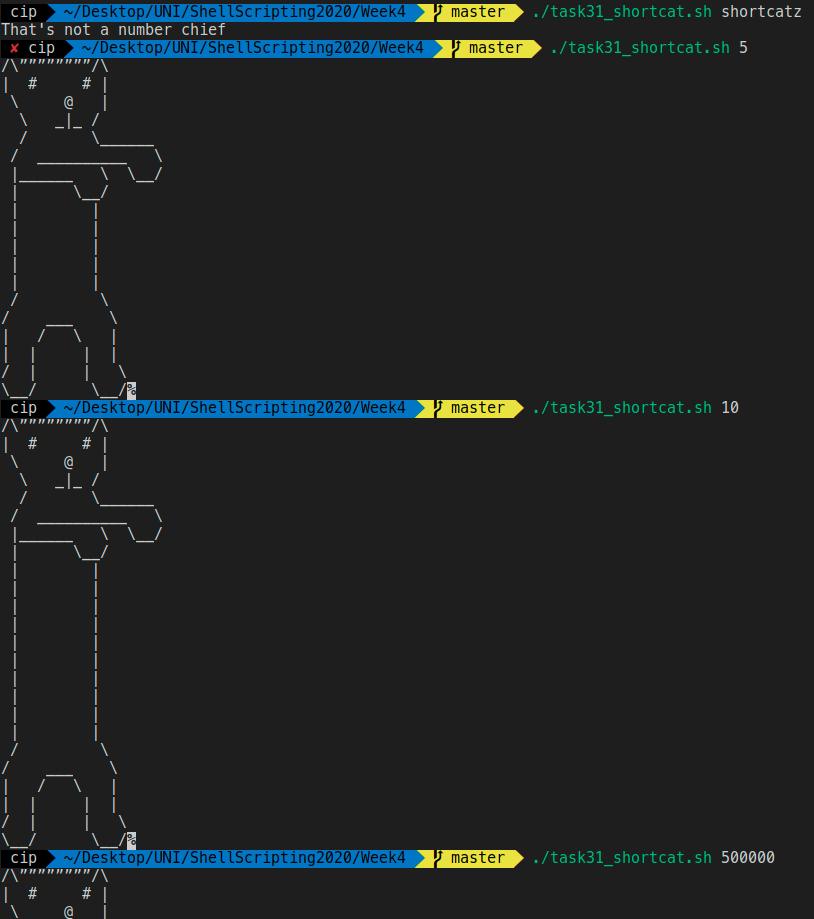
\includegraphics[width=14cm]{img/31.png}
		\end{figure}
	
		\newpage
		Contents of the \texttt{task31\_shortcat.sh} file:
		\VerbatimInput{../task31_shortcat.sh}

	\item \textbf{Plotting}
	
		Contents of the \texttt{task32\_create\_random\_data.sh} file:
		\VerbatimInput{../task32_create_random_data.sh}

		Contents of the \texttt{task32\_create\_random\_data.p} file:
		\VerbatimInput{../task32_create_random_data.p}
		
		\newpage
		Output of the plot:
		\begin{figure}[h!]
			\centering
			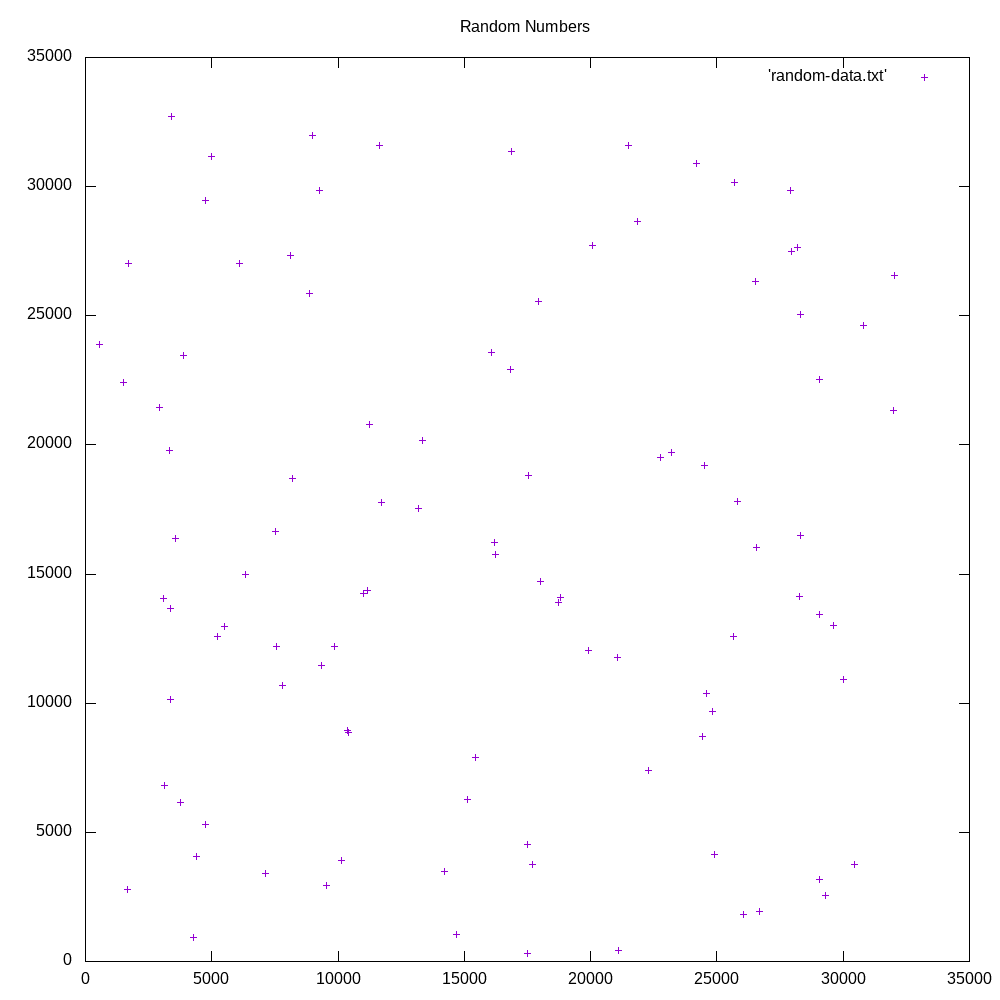
\includegraphics[width=14cm]{../task32_create_random_data}
		\end{figure}

	\item \textbf{Let's plot some real data points}

		Contents of the \texttt{task33\_plot\_real\_data.sh} file:
		\VerbatimInput{../task33_plot_real_data.sh}

		Contents of the \texttt{task33\_plot\_real\_data.txt} file:
		\VerbatimInput{../task33_plot_real_data.txt}

		Contents of the \texttt{task33\_plot\_real\_data.p} file:
		\VerbatimInput{../task33_plot_real_data.p}
		
		Contents of the \texttt{task33\_plot\_real\_data.eps} file, output of the execution:
		\begin{figure}[h!]
			\centering
			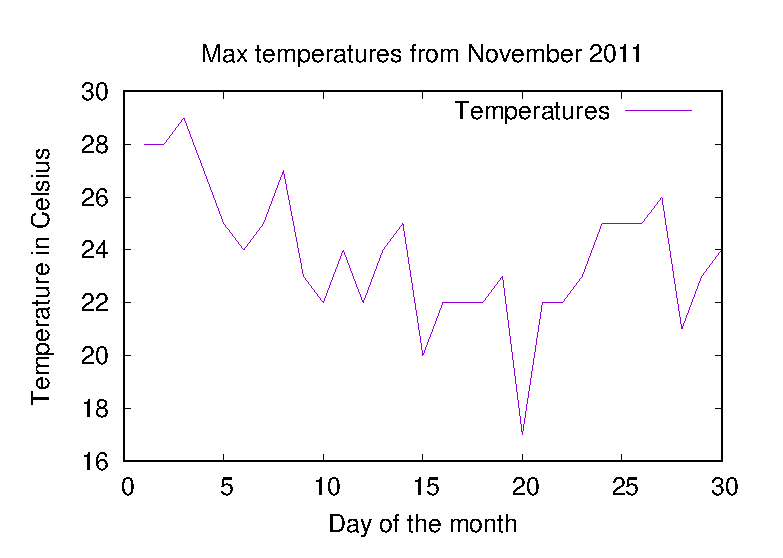
\includegraphics[width=10cm]{../task33_plot_real_data.eps}
		\end{figure}		

	\item \textbf{Let's put some context}
	
		Contents of the \texttt{task34\_plot\_min-max-temps-2011-11.sh} file:
		\VerbatimInput{../task34_plot_min-max-temps-2011-11.sh}

		Contents of the \texttt{task34\_plot\_min-max-temps-2011-11.txt} file:
		\VerbatimInput{../task34_plot_min-max-temps-2011-11.txt}

		Contents of the \texttt{task34\_plot\_min-max-temps-2011-11.p} file:
		\VerbatimInput{../task34_plot_min-max-temps-2011-11.p}
		
		Contents of the \texttt{task34\_plot\_min-max-temps-2011-11.eps} file, output of the execution:
		\begin{figure}[h!]
			\centering
			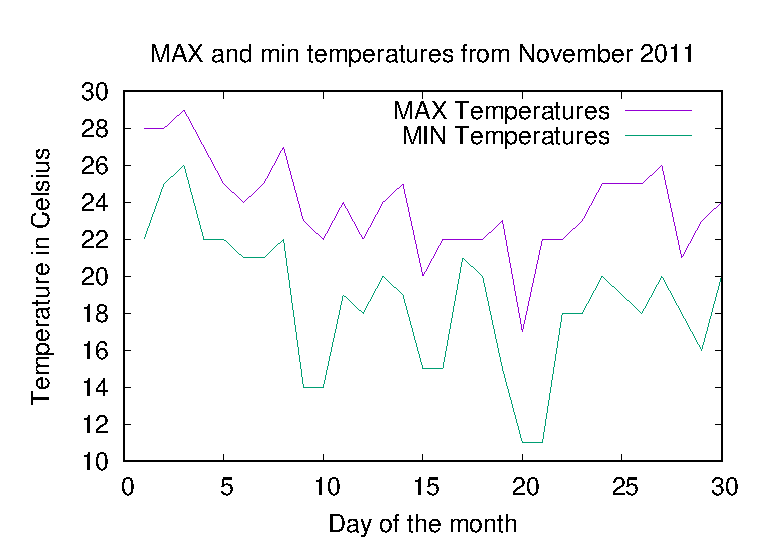
\includegraphics[width=10cm]{../task34_plot_min-max-temps-2011-11.eps}
		\end{figure}		

	\item \textbf{Let's generalize}
	
		Contents of the \texttt{task35\_plot\_min-max-tempsgeneralized.sh} file:
		\VerbatimInput{../task35_plot_min-max-temps_generalized.sh}
		
		Contents of the \texttt{task35\_plot\_min-max-tempsgeneralized.txt} file:
		\VerbatimInput{../task35_plot_min-max-temps_generalized.txt}
		
		Contents of the \texttt{task35\_plot\_min-max-tempsgeneralized.p} file:
		\VerbatimInput{../task35_plot_min-max-temps_generalized.p}
	
		Contents of the \texttt{task35\_plot\_min-max-temps\_generalized.eps} file, output of the execution:
		\begin{figure}[h!]
			\centering
			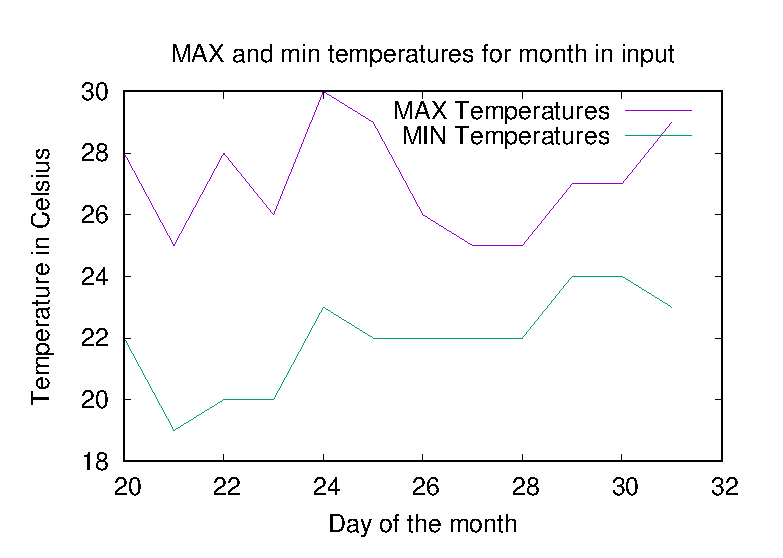
\includegraphics[width=10cm]{../task34_plot_min-max-temps_generalized.eps}
		\end{figure}		
	
	\item \hl{\textbf{Let's make more refined commands}}
	
\end{enumerate}

\end{document}